\documentclass[tikz]{standalone}
\usepackage{underscore}

\usetikzlibrary{fit,arrows.meta}

\tikzset{
  data/.style={circle, fill=black},
  data label/.style={font=\ttfamily},
  data box/.style={draw=black, font=\ttfamily},
  next/.style={circle, fill=black},
  next label/.style={font=\ttfamily},
  prev/.style={circle, fill=black},
  prev label/.style={font=\ttfamily},
  node label/.style={draw=black, prefix after command={\pgfextra{\tikzset{every label/.style={font=\bfseries\ttfamily}}}}},
  link/.style={arrows={-Latex}},
  new link/.style={arrows={-Latex}, blue},
  HEAD/.style={font=\ttfamily},
  NULL/.style={font=\ttfamily}
}


\tikzset{
  pics/llnode/.style args={#1/#2}{
    code = {
      \node[prev] at (0,1.25) (#1 prev) {};
      \node[prev label] at (0,1.75) (#1 prev label) {prev\strut};

      \node[next] at (0,0) (#1 next) {};
      \node[next label] at (0,0.5) (#1 next label) {next\strut};

      \node[data] at (0,-1.25) (#1 data) {};
      \node[data label] at (0,-0.75) (#1 data label) {data\strut};

      \node[node label,fit={(#1 prev) (#1 prev label) (#1 next) (#1 next label) (#1 data) (#1 data label)},label={[label distance=0.25cm]#2}] (#1) {};
    }
  }
}


\begin{document}

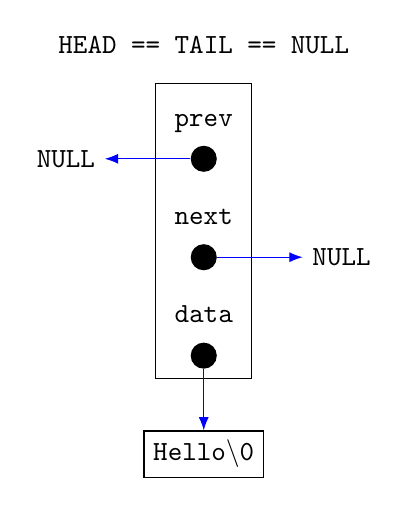
\begin{tikzpicture}
  \pic at (0,0) {llnode=node_ptr/{HEAD == TAIL == NULL}};

  \node[NULL] at (-1.75, 1.25) (prev NULL) {NULL};
  \node[NULL] at ( 1.75, 0) (next NULL) {NULL};

  \node[data box] at (0,-2.5) (Hello) {Hello\textbackslash0};

  \draw[new link] (node_ptr data) -- (Hello);
  \draw[new link] (node_ptr prev) -- (prev NULL);
  \draw[new link] (node_ptr next) -- (next NULL);
\end{tikzpicture}


\end{document}
